\section{Antecedentes}
 
El punto de partida para la presente reingeniería es el sistema operativo hasta el periodo 2023, consolidado mediante los trabajos de \cite{aguilera2022} y \cite{zhou2023}. En particular, la carpeta \texttt{RutaCritica} contiene el prototipo y la labor del equipo responsable que aportaron conceptos formales y heurísticos clave —los cuales han sido cuidadosamente respetados y extendidos en \texttt{Quickshift}—. A continuación se articula una descripción técnica ampliada, ilustrada con una gráfica conceptual de complejidad.

\subsection{Modelo algorítmico legado}

El núcleo del sistema anterior se basó en la resolución del problema del \textbf{Clique de Peso Máximo}. La representación del dominio era directa: cada sección se modela como un nodo; las aristas representan compatibilidades temporales (no topes) y la idoneidad de una sección se expresa mediante un peso numérico.

La generación del peso combina factores derivados del análisis PERT (holgura, criticidad), la posición relativa en la malla (número correlativo) y preferencias locales (profesor, compactación), implementándose en \texttt{get\_clique\_max\_pond.py} mediante la concatenación CC+UU+KK+SS descrita en los anexos de código.

\subsection{Limitaciones estructurales y rendimiento}

El enfoque de \texttt{RutaCritica} es conceptualmente sólido y aportó una base práctica imprescindible; sin embargo, al llevar el prototipo a contextos de producción se identificaron desafíos operativos y de escalado que motivaron optimizaciones adicionales. Entre los aspectos observados se encuentran:
\begin{itemize}
  \item \textbf{Elección de estrategia (poda posterior):} En fases exploratorias se optó por generar conjuntos amplios y aplicar poda posterior para garantizar exhaustividad y facilitar el análisis. Esta decisión, razonable en la etapa de investigación y diagnóstico, ofrece hoy oportunidades de optimización cuando el objetivo es latencia reducida en producción.
  \item \textbf{Crecimiento combinatorio y coste computacional:} El coste de búsqueda aumenta de forma muy rápida con el número de secciones; con la oferta actual (≈692 secciones) las ejecuciones exhaustivas llegan a ser costosas en tiempo y memoria.
  \item \textbf{Heterogeneidad y mantenimiento de datos:} Las variaciones administrativas en códigos y formatos incrementan la necesidad de normalización y mapeo de equivalencias para asegurar trazabilidad entre historial y oferta.
\end{itemize}

Para ilustrar el impacto en tiempo de cómputo y el punto donde una heurística acotada aporta ventaja operativa, incluimos una gráfica conceptual comparativa (eje vertical: tiempo de CPU; eje horizontal: número de secciones).

\begin{figure}[H]
  \centering
  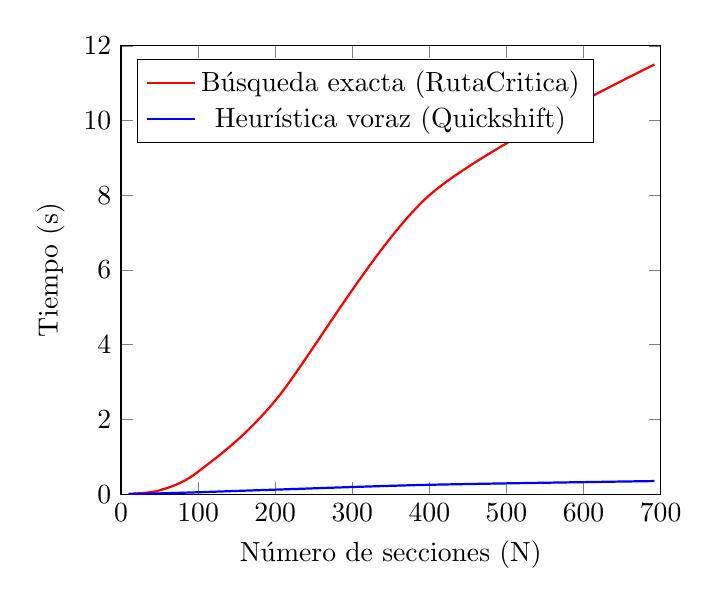
\begin{tikzpicture}
    \begin{axis}[xlabel={Número de secciones (N)}, ylabel={Tiempo (s)}, xmin=0, xmax=700, ymin=0, ymax=12, legend pos=north west]
      % curva exponencial (conceptual)
      \addplot[smooth, thick, red] coordinates {(10,0.01) (50,0.1) (100,0.6) (200,2.5) (400,8.0) (692,11.5)};
      \addlegendentry{Búsqueda exacta (RutaCritica)}
      % curva heurística (conceptual)
      \addplot[smooth, thick, blue] coordinates {(10,0.005) (50,0.02) (100,0.05) (200,0.12) (400,0.25) (692,0.35)};
      \addlegendentry{Heurística voraz (Quickshift)}
    \end{axis}
  \end{tikzpicture}
  \caption{Comparativa ilustrativa de escalado temporal entre la búsqueda exhaustiva (prototipo) y la heurística voraz (optimización de producción). Los valores son orientativos y dependen de la implementación y la plataforma.}
\end{figure}

\subsection{RutaCritica: definición y flujo operativo}
La implementación original disponible en \texttt{RutaCritica} articula el proceso en etapas reproducibles:
\begin{enumerate}
  \item \textbf{Extracción y normalización de datos:} \texttt{extract\_data.py} parsea las fuentes (Excel/CSV), normaliza nombres y construye la lista de secciones con atributos (horario, profesor, código, secci\'on).
  \item \textbf{Análisis PERT:} \texttt{rutaCritica.py} construye un DAG de prerrequisitos y calcula ES/EF/LS/LF/H para identificar ramos cr\'iticos y holguras, información usada en la ponderación.
  \item \textbf{Construcción del grafo ponderado:} \texttt{get\_clique\_max\_pond.py} crea un grafo (NetworkX) con nodos ponderados por la función de prioridad; las aristas representan compatibilidades horarias.
  \item \textbf{Búsqueda de cliques ponderados:} se aplica el algoritmo de clique máximo ponderado (o una heurística local) para obtener soluciones candidatas.
  \item \textbf{Post‑procesado y presentación:} selección de soluciones, poda a carga máxima, ordenamiento por criterios de usabilidad y exportación a JSON/CSV.
\end{enumerate}

\subsection{Rigor metodológico y documentación necesaria}
Para garantizar reproducibilidad y trazabilidad se recomienda que la documentación incluya:
\begin{itemize}
  \item Formato de entrada y ejemplos minimalistas (plantillas Excel/CSV).
  \item Fórmulas de ponderación y ejemplos numéricos que expliquen CC, UU, KK y SS.
  \item Parámetros de ejecución (n\'umero de semillas, iteraciones, límites de tiempo) y valores por defecto para cada script.
  \item Métricas y procedimientos de evaluación: perfil de latencias, uso de memoria, tasa de soluciones v\'alidas, cobertura frente a equivalencias.
\end{itemize}

\subsection{Recomendaciones}
Se recomienda mantener en el anexo del informe tablas cortas que describan los scripts clave del prototipo \texttt{RutaCritica} (\texttt{extract\_data.py}, \texttt{get\_clique\_max\_pond.py}, \texttt{rutaCritica.py}), parámetros de ejecución y un conjunto de pruebas reproducibles que permitan verificar la equivalencia funcional con \texttt{Quickshift} sobre casos representativos.

